%%%% PROCESAR con PdfLaTeX !!!!!


\documentclass[12pt]{book}
\usepackage{geometry}\geometry{top=2cm,bottom=2cm,left=3cm,right=3cm}
\usepackage{amssymb}
\usepackage{amsmath}
\usepackage{graphicx}
\usepackage{txfonts}
%\usepackage{hyperref}
\usepackage[hidelinks]{hyperref}
\usepackage[spanish]{babel}
\setcounter{tocdepth}{3}
\usepackage[usenames]{color}

\usepackage[hidelinks]{hyperref}
\hypersetup{
    colorlinks=true,
    linkcolor=black,
    filecolor=magenta,      
    urlcolor=cyan,
    pdftitle={Sharelatex Example},
    bookmarks=true,
%    pdfpagemode=FullScreen,
}


\begin{document}
\thispagestyle{empty}

\begin {center}

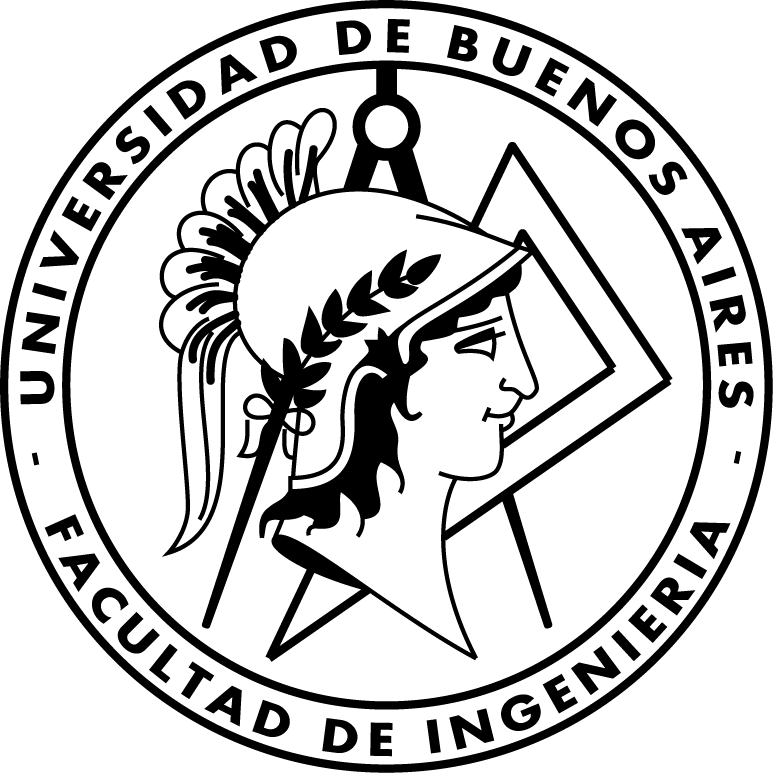
\includegraphics[scale=.4]{Logo-fiuba_big.png}

\medskip
UNIVERSIDAD DE BUENOS AIRES

Facultad de Ingenier\'ia

Departamento de Computaci\'on


\vspace{3cm}


\textbf{\large 7510 T\'ecnicas de Diseño}

\vspace{2cm}


Este es un modesto aporte para los alumnos de la f\'acultad de ingenier\'ia  de la UBA de las carreras de licenciatura en an\'alsis de sistemas e ingenier\'ia inform\'atica.
De ninguna man\'era pretende ser una gu\'ia de estudio, ni remplaza las clases presenciales, el material oficial de la catedra esta disponible en el web site de la m\'ateria.
\\
\url{http://materias.fi.uba.ar/7510/}

\end {center}


\vspace{2.5cm}

\noindent Autor:\,	Isaac Edgar Camacho Ocampo
 
\noindent Carrera:\,	Licenciatura en An\'alisis de sistemas

\vspace{1cm}

\vspace{1cm}

\noindent Buenos Aires, 2019

\newpage


\tableofcontents
\chapter{Introducción}En el mundo real existen fenomenos que podemos conocer atravez de la experiencia, y la ciencia ha tratado a lo largo de la historia de predecir tales acontecimientos, por ejemplo una tormenta una sequia etc. 
\\
Debido a la complejidad de la realidad es comun que los cientificos trabajen con simplificaciones que llamaremos modelos, que utilizamos para trabajar, es decir que trataremos de reproducir fenomenos y trataremos de predecir el resultado.
\\
\section{Modelos probabilísticos}Para los problemas en los que se quiere averiguar las chances de algún resultado la física por ejemplo ha elaborado modelos que bajo las mismas condiciones iniciales  nos garantiza un único resultado, sin embargo estos modelos son muy complicados porque toman en cuenta muchos factores, por ejemplo si tenemos en cuenta al lanzar una moneda el clima, la fuerza aplicada, la temperatura etcétera, el modelo nos brindará mucha información pero el manejo de toda esa información es muy dificil, en cambio  sí construimos un modelo bajo el principio de indiferencia, perdemos información pero ganamos en simplicidad, entonces nuestro trabajo será el de, a partir de un modelo simple obtener información relevante.

\section{Experimento}
Es cualquier acto en el cual el resultado exacto no se puede predecir con certeza. Todos los ejemplos que vimos, la moneda, las cartas, los dados, etc., son experimentos en este sentido. Existen dos tipos de experimentos:
\begin{itemize}
\item Deterministicos: cuando bajo las mismas condiciones iniciales, se obtienen iguales resultados y de esto se encarga la fisica, por ejemplo con la ecuacion horaria $x_0 = x_i + v_0 t$

\item Estocasticos o aleatorios: Cuando bajo las mismas condiciones iniciales se obtienen varios resultados, por ejemplo \textbf{determinar la cantidad de lluvia en una zona} de esto se ocupa la Probabilidad.
\end{itemize}
\section{¿Que es la probabilidad?}
La misma nace con los juegos de azar, intuitivamente la podemos definir como:
\textbf{La probabilidad es el grado de certeza de que ocurrira un determinado resultado en un experimento aleatorio dado, cuanto mayor sea la probabilidad, mayor es el grado de certeza de que ocurrira dicho resultado} en otras palabras es la chance de que salga uno u otro resultado.
\\
por ejemplo:
\begin{itemize}
\item Que chance tengo de sacarme un 8 en un examen?
\item Que chance tengo de acertar la loteria?
\item que chances hay en sacar poker de ases?
\end{itemize}
\section{Intuici\'on}
Sin saber nada, ¿cómo podríamos calcular la probabilidad de algo?, simplemente hacemos, casos favorables sobre casos totales. Cuando tiramos una moneda la probabilidad de sacar cara, es 50\%, porque solo hay dos resultados posibles.
\section{Principio de indiferencia}
Si no hay razones por las cuales sospechar que un resultado particular tiene más chances de ocurrir que los demás, entonces todos los resultados deben tener la misma probabilidad.
\\
\\
Esta es una manera intuitiva de calcular las probabilidades donde todos los resultados tienen la misma chance de ocurrir y el conjunto de todos los resultados posibles los llamaremos equiprobables (igual probabilidad), Muchos autores las llaman \textbf{distribución uniforme discreta}. 

\subsubsection{Ley de los grandes números y frecuencia relativa}
Cuando decimos que  al lanzar una moneda la probabilidad  de sacar cara es un medio, estamos asumiendo que los dos resultados posibles tienen las mismas chances de salir, pero también se puede justificar de otra forma, preguntándose ¿qué pasa a la larga? o en muchas repeticiones del experimento.
¿Qué pasa si esa misma moneda la tiró 10 veces?  Lo más Sensato sería pensar que 5 veces saldrá cara y 5 veces salga seca, si repito el experimento un millón de veces la conclusión sería la misma.
\\
\\
Sí repetimos el experimento muchas veces, es decir, un número grande de repeticiones, es muy probable que la frecuencia relativa de caras, esté cercana al un medio, esta definición tiene el problema de ser recursiva.
\section{Espacio muestral}
Es el conjunto de todos los resultados posibles de un experimento. Los elementos del espacio muestral se denota usualmente por la letra griega $\omega $ (omega minúscula) y se llaman eventos simples o elementales.
\section{Evento}
Es una subcolección de resultados posibles de un experimento (un evento A es un subconjunto del espacio muestral $ \Omega $ ). Si el resultado observado es un cierto $ \omega$ perteneciente a un evento A (esto lo escribimos $ \omega \in A $), decimos entonces que A ha ocurrido.

\section{Cardinal}
es el número de elementos de un evento, lo escribimos $ \vert A \vert| $ . Con esta notación la probabilidad de un evento A es $P ( A ) = | A | / | \Omega |$

\section{Complemento}
 consiste en todos los eventos simples que no pertenecen a A. Este evento lo denotaremos por


\section{Intersección}Sxpresa la condición de que ambos A y B ocurran simultáneamente. Este evento se escribe Cuando dos eventos no tienen elementos en común, decimos que son incompatibles o disjuntos y escribimos $A \cap B = \emptyset $. En palabras, esto quiere decir que si A ocurre, B no puede ocurrir, y viceversa.


\section{Unión}expresa la condición de que A o B ocurran. Se entiende la conjunción o en el sentido amplio, una cosa o la otra o ambas. Este evento se escribe


\section{Inclusión} expresa la condición de que A implica B. Esto lo escribimos $A \subset B$.


\section{Diferencia}: expresa la condición A pero no B. Se escribe A \ B.


Un determinado problema o proceso aleatorio puede tener múltiples modelos y esto nos lleva a pensar que el principio de indiferencia puede fallar.
\\
\\
Un escenario posible es el siguiente: si lanzamos dos dados y miramos la suma de los resultados, podríamos decir que los casos posibles son los números del 2 al 12, pero parece menos probable que salga un 2 a que salga un 7. En este caso sería mejor aplicar el principio a los pares de números que representan los resultados de cada dado. Este tipo de ejemplos es típico, los resultados posibles que nos interesan no son equiprobables, pero se pueden formular a partir de otros que sí lo son. Lo más importante de construir un modelo probabilístico Es asignar probabilidades.


\chapter{Variable aleatoria}
Al trabajar hasta este momento con experimentos aleatorios, lo que hicimos fue encontrar un espacio muestral y calcular el cardinal de dicho espacio para luego a cada evento del espacio muestral, asociarle un número que llamamos probabilidad, sin embargo hay experimentos en los que es extremadamente difícil calcular el cardinal del espacio muestral y peor aún ni siquiera es necesario calcularlo. \\
\\
Para resolver esos problemas aparecen las variables aleatorias veamos el siguiente ejemplo.
\\ \\
en un experimento biológico se miden la altura en centímetros de 60 plantas, a partir de sus mediciones conformamos una tabla, lo que en definitiva buscamos es poder predecir la altura que tendrá una planta después de 6 meses.
\\ \\
\textbf{¿Qué es lo que determina la altura de las plantas?}
Bueno aquí podemos decir que intervienen el clima los nutrientes del suelo, la genética, la biodiversidad, etcétera, etcétera, 
como vemos la cantidad de factores intervinientes no es trivial, entonces hallar un espacio muestral asociado a este experimento resulta bastante complicado porque tendríamos que contemplar todas las historias de vida de cada una de las plantas.
\\ \\
Si por alguna razón podemos construir un espacio muestral que refleja nuestra experimento, queda algo más complicado que es ¿como asignó probabilidades? es decir a cada evento del espacio muestral ¿cómo le asignó una probabilidad?, ¿qué es lo que influye más?, ¿la genética los nutrientes, el clima?.
\\ \\
Entonces podríamos preguntarnos ¿cuál es la probabilidad de que alcance determinada altura si tuvo determinados nutrientes en un clima cálido y con determinada genética?.
\\ \\
Uno puede pensar que es casi imposible hacer modelo matemático que refleje la probabilidad de que una planta alcance determinada altura sin embargo se puede gracias a la variables aleatorias, la idea es la siguiente, en realidad no me importan todas las determinadas condiciones de crecimiento de la planta es decir no me importan cómo se relacionan, el clima con la biodiversidad, etcétera,
\\
Sí definimos X = como la altura de una planta \\ \\

No necesito toda la información del contexto lo único que necesito es saber con qué probabilidad X va a tomar determinados valores de altura, entonces no necesito calcular el espacio muestral y mucho menos calcular la probabilidad de cada evento del espacio, entonces sólo necesito saber cuál es la probabilidad de que por ejemplo X valga 21 cm y este es un evento mucho más sencillo.
\\ \\
Las variables aleatorias son funciones que toman elementos del espacio muestral y asignan un número real, podemos decir también que X va del espacio de todas las historias de vida posibles a los reales y lo único que me interesa conocerte de X es con qué probabilidad toma cada uno de los valores, eso es lo que se llama la distribución de X, entonces no necesitamos conocer, ni el espacio muestral, ni las probabilidades de cada evento de es espacio, lo único que necesitamos es la distribución de esta variable.
\\ \\
\textbf{La distribuciones de X son qué valores pueden tomar y con qué probabilidad lo hace}

Variable aleatoria
Es una función del espacio muestral en los reales y puede haber de dos tipos variables discretas y continuas las discretas son aquellas que toman valores enteros contables es decir numerables y las continuas miden por ejemplo la velocidad del viento la cantidad de agua en una lluvia

una regla para darse cuenta si un modelo es continuo y discreto es preguntarse si estoy contando cosas o midiendo cosas

\section{Teoría clásica}
\subsection{Definición de variables}
\subsection{Pruebas y refutaciones}
\section{Hipótesis}
\chapter{Resultados}
\section{Simulación de resultados}
\subsection{Suposiciones}
\subsection{Modelos}
\section{Resultados preliminares}
\section{Resultados postprocesados}
\subsection{Valores atípicos}
\subsection{Correlaciones}
\chapter{Conclusiones}
\end{document}
